\documentclass{scrreprt}
\usepackage{amsmath}
\usepackage{listings}
\usepackage{array}
\usepackage{tikz} 
\usepackage{underscore}
\usepackage[bookmarks=true]{hyperref}
\usepackage[utf8]{inputenc}
\usepackage[english]{babel}
\usepackage{enumitem}
\usepackage[a4paper, margin=1in]{geometry}
\usetikzlibrary{shapes, arrows.meta, positioning, backgrounds}

% Define styles for different node types
\tikzstyle{startstop} = [rectangle, rounded corners, minimum width=3cm, minimum height=1cm, text centered, draw=black, fill=red!30]
\tikzstyle{process} = [rectangle, minimum width=3.5cm, minimum height=1cm, text centered, draw=black, fill=blue!30]
\tikzstyle{arrow} = [thick,->,>=stealth]

% Define stickman style
\tikzset{
    stickman/.pic={
        % Head
        \draw[fill=gray] (0,0.6) circle (0.3cm);
        % Body
        \draw[line width=0.5mm] (0,0.3) -- (0,-0.6);
        % Arms
        \draw[line width=0.5mm] (-0.4,0.3) -- (0.4,0.3);
        % Legs
        \draw[line width=0.5mm] (0,-0.6) -- (-0.4,-1.2);
        \draw[line width=0.5mm] (0,-0.6) -- (0.4,-1.2);
    }
}

% Hyperref settings
\hypersetup{
    pdftitle={Software Requirement Specification},
    pdfauthor={Jean-Philippe Eisenbarth},
    pdfsubject={TeX and LaTeX},
    pdfkeywords={TeX, LaTeX, graphics, images},
    colorlinks=true,
    linkcolor=blue,
    citecolor=black,
    filecolor=black,
    urlcolor=purple,
    linktoc=page
}

% Set extra row height and padding
\setlength{\extrarowheight}{4pt}
\renewcommand{\arraystretch}{1.5}

\begin{document}

\begin{titlepage}
    \centering
    
\includegraphics[width=0.5\textwidth]{./logo.png} 
    \vspace{1cm}

    \textbf{Department of Computer Science and Engineering}\\
    Premier University
    \vspace{1cm}

    \huge \textnormal{EEE 371: Microprocessors \& Microcontrollers }
    \vspace{1in} 

    \Large \textnormal{Title: Complex Engineering Problem}
    \vspace{0.5in} 

    \large
    \textbf{Submitted by:}
    \vspace{0.5cm}

    \renewcommand{\arraystretch}{1.5} 
    \begin{tabular}{|p{0.4\textwidth}|p{0.6\textwidth}|}
        \hline
        \textbf{Name} & Mohammad Hafizur Rahman Sakib \\
        \hline
        \textbf{ID} & 0222210005101118 \\
        \hline
        \textbf{chapter} & C \\
        \hline
        \textbf{Session} & Spring 2024 \\
        \hline
        \textbf{Semester} & 5th Semester \\
        \hline
        \textbf{Submission Date} & 14.09.2024 \\
        \hline
    \end{tabular}
    \vspace{1cm}

    \begin{minipage}[t]{0.48\textwidth}
        \textbf{Submitted to:}\\
        Mahmudul Hassan Emon\\
        Lecturer, Department of CSE\\
        Premier University\\
        Chittagong
    \end{minipage}%
    \hfill
    \begin{minipage}[t]{0.48\textwidth}
        \raggedleft
        \textbf{Remarks}\\
        \vspace{0.5cm} % Adjust vertical space for remarks
        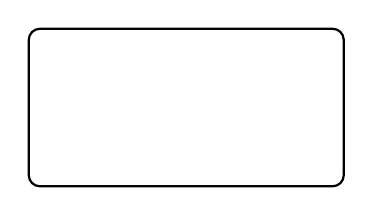
\begin{tikzpicture}
            \draw[thick, rounded corners] (0,0) rectangle (4,2);
        \end{tikzpicture}
    \end{minipage}

    \date{\today}
    \vfill
\end{titlepage}

\section*{Problem Statement}
Urban traffic congestion, especially at interchapters, is a growing issue due to increasing population. This project involves designing an Autonomous Traffic Management System (ATMS) for a three-way interchapter, aiming to improve traffic flow, reduce congestion, and enhance safety using embedded systems and smart infrastructure.

\section*{Abstract}
The Autonomous Traffic Management System (ATMS) is an advanced solution designed to tackle urban traffic congestion by integrating sensors, embedded systems, and real-time traffic data. It continuously monitors vehicle movement and traffic patterns at intersections, allowing it to dynamically adjust traffic signals based on current conditions. This real-time responsiveness significantly improves traffic flow, reduces congestion, and minimizes vehicle idling, leading to a direct decrease in fuel consumption and harmful emissions.

The Autonomous Traffic Management System (ATMS)** is an innovative solution aimed at reducing urban traffic congestion by using sensors, embedded systems, and real-time data. It continuously monitors traffic at intersections, dynamically adjusting signals to improve flow, reduce congestion, and minimize vehicle idling, which cuts fuel consumption and emissions.
A key feature of ATMS is its ability to prioritize emergency vehicles, such as ambulances, by overriding regular signals to provide them with a clear path, improving emergency response times. The system also promotes eco-friendly transportation by reducing stop-and-go traffic, lowering emissions, and enhancing the commuter experience.

Additionally, ATMS improves road safety by coordinating traffic signals with autonomous vehicles through Vehicle-to-Infrastructure (V2I) communication, reducing accidents. By integrating advanced technology and real-time monitoring, ATMS addresses critical issues like congestion, emissions, and emergency response, contributing to a safer and more sustainable urban transport system.
\section*{Required Equipment}

The Autonomous Traffic Management System (ATMS) relies on several critical components. The key equipment required includes:

\begin{itemize}
    \item \textbf{Traffic Cameras}
    \item \textbf{LIDAR Sensors}
    \item \textbf{Pressure Sensors}
    \item \textbf{Central Control Unit (CCU)}
    \item \textbf{Vehicle-to-Infrastructure (V2I) Communication System}
    \item \textbf{Emergency Vehicle Preemption System}
    \item \textbf{Power Supply and Backup}
    \item \textbf{Data Storage and Management}
    \item \textbf{Maintenance and Monitoring Systems}
    \item \textbf{Security Measures}
\end{itemize}

\section*{Proposed Solution}

The Autonomous Traffic Management System (ATMS) is designed to revolutionize the management of urban traffic at intersections by leveraging advanced technology, real-time data processing, and intelligent decision-making algorithms. The proposed solution focuses on optimizing traffic flow, reducing congestion, and enhancing overall safety. Below is a detailed breakdown of the key components and processes involved in the ATMS.

\subsection*{1. Real-Time Data Collection and Monitoring}

The foundation of the ATMS lies in its ability to collect and monitor real-time traffic data at the intersection. This is achieved through an array of sensors, including traffic cameras, LIDAR sensors, and pressure sensors. Each type of sensor plays a specific role:

\begin{itemize}
    \item \textbf{Traffic Cameras:} 
    Traffic cameras are installed at various angles around the intersection to capture visual data on vehicle count, speed, and flow. The cameras provide continuous monitoring, allowing the system to detect real-time changes in traffic conditions.

    \item \textbf{LIDAR Sensors:} 
    LIDAR sensors create detailed 3D maps of the intersection, offering precise information on the position, speed, and size of vehicles. This data is crucial for tracking vehicle movements and predicting potential congestion points.

    \item \textbf{Pressure Sensors:} 
    Pressure sensors embedded in the road surface detect the presence of vehicles by measuring the pressure exerted on them. This information helps determine vehicle waiting times at signals and the number of vehicles in each lane.
\end{itemize}

All collected data is transmitted to the Central Control Unit (CCU) in real-time for processing.

\subsection*{2. Central Control Unit (CCU) and Data Processing}

The CCU serves as the brain of the ATMS, processing the incoming data from sensors and making decisions to manage traffic flow efficiently. The CCU uses embedded systems technology, which provides a compact, reliable, and energy-efficient platform for data processing.

\begin{itemize}
    \item \textbf{Data Analysis:} 
    The CCU employs advanced algorithms to analyze the real-time data. It assesses traffic density, vehicle speeds, and waiting times at the intersection. This analysis allows the system to identify patterns and predict congestion before it occurs.

    \item \textbf{Signal Timing Optimization:} 
    Based on the analyzed data, the CCU dynamically adjusts traffic signal timings. For example, if the system detects an increase in vehicle volume from a particular direction, it can extend the green light duration for that direction to alleviate congestion.

    \item \textbf{Predictive Analytics:} 
    The CCU uses machine learning algorithms to learn from historical traffic data. This allows the system to make more accurate predictions about future traffic conditions and optimize signal timings proactively, rather than reactively.
\end{itemize}

The ability to process and respond to real-time data enables the ATMS to maintain smooth traffic flow and minimize delays.

\subsection*{3. Vehicle-to-Infrastructure (V2I) Communication}

To enhance traffic management, the ATMS integrates a Vehicle-to-Infrastructure (V2I) communication system. V2I communication enables direct interaction between the ATMS and vehicles, particularly autonomous vehicles equipped with this technology.

\begin{itemize}
    \item \textbf{Data Exchange:} 
    Through V2I communication, vehicles can share data with the ATMS, such as their speed, route, and estimated arrival time at the intersection. In return, the ATMS can provide vehicles with information about upcoming signal changes, traffic conditions, and potential hazards.

    \item \textbf{Coordination with Autonomous Vehicles:} 
    The ATMS can coordinate with autonomous vehicles to optimize their movement through the intersection. For example, it can adjust signal timings to ensure that autonomous vehicles pass through without stopping, reducing fuel consumption and improving traffic flow.

    \item \textbf{Enhanced Safety:} 
    V2I communication also enhances safety by enabling the ATMS to send alerts to vehicles about potential collisions or obstacles at the intersection. This allows drivers or autonomous systems to take preventive actions, reducing the likelihood of accidents.
\end{itemize}

V2I communication is a key component in making the ATMS a forward-looking, future-proof system that can adapt to the increasing presence of autonomous vehicles on the road.

\subsection*{4. Emergency Vehicle Preemption System}

A crucial feature of the ATMS is its ability to prioritize emergency vehicles, such as ambulances and fire trucks, ensuring they can navigate intersections quickly and safely.

\begin{itemize}
    \item \textbf{Detection and Communication:} 
    The system detects the presence of an emergency vehicle through V2I communication or GPS tracking. Once detected, the ATMS immediately takes action to clear the path for the emergency vehicle.

    \item \textbf{Signal Override:} 
    The ATMS temporarily overrides normal traffic signal operations to give the emergency vehicle a green light, while holding all other traffic at a red light. This ensures the emergency vehicle can pass through the intersection without delay.

    \item \textbf{Resumption of Normal Operations:} 
    After the emergency vehicle has cleared the intersection, the ATMS quickly returns to normal signal operations, minimizing disruption to overall traffic flow.
\end{itemize}

This preemption system significantly improves emergency response times, potentially saving lives by allowing first responders to reach their destinations more quickly.

\subsection*{5. Continuous Monitoring and Optimization}

The ATMS is designed to operate continuously, monitoring traffic conditions and making real-time adjustments to optimize performance. To ensure the system remains effective over time, it includes several key features:

\begin{itemize}
    \item \textbf{Real-Time Feedback Loop:} 
    The system continuously monitors the effectiveness of its signal timing decisions. If the desired improvements in traffic flow are not achieved, the CCU can quickly adjust the parameters and re-optimize signal timings.

    \item \textbf{Machine Learning Integration:} 
    By incorporating machine learning algorithms, the ATMS can learn from past traffic patterns and improve its decision-making processes over time. This allows the system to adapt to changing traffic conditions, such as seasonal variations or special events, without requiring manual reconfiguration.

    \item \textbf{Scalability and Flexibility:} 
    The ATMS is designed to be scalable, allowing it to be expanded to additional intersections as needed. It is also flexible, enabling easy integration of new technologies or updates as they become available.
\end{itemize}

This continuous optimization ensures that the ATMS remains a robust and adaptive solution for urban traffic management.

\subsection*{7. Future Expansion and Development}

While the initial implementation of the ATMS focuses on a single three-way intersection, the system is designed with future expansion in mind.

\begin{itemize}
    \item \textbf{Integration with Other Intersections:} 
    The system can be expanded to manage multiple intersections, creating a coordinated network of traffic signals across a larger area. This would allow for more comprehensive traffic management, optimizing flow across an entire district or city.

    \item \textbf{Incorporation of Machine Learning for Predictive Traffic Management:} 
    As the system expands, incorporating more advanced machine learning algorithms could enhance its predictive capabilities. This would allow the ATMS to anticipate traffic patterns further in advance and make proactive adjustments to signal timings.

    \item \textbf{Collaboration with Smart City Initiatives:} 
    The ATMS can be integrated into broader smart city initiatives, working in conjunction with other infrastructure systems, such as public transportation, to create a more efficient and interconnected urban environment.
\end{itemize}

This focus on future expansion ensures that the ATMS remains a vital component of urban infrastructure as cities grow and evolve.


\begin{center}
    {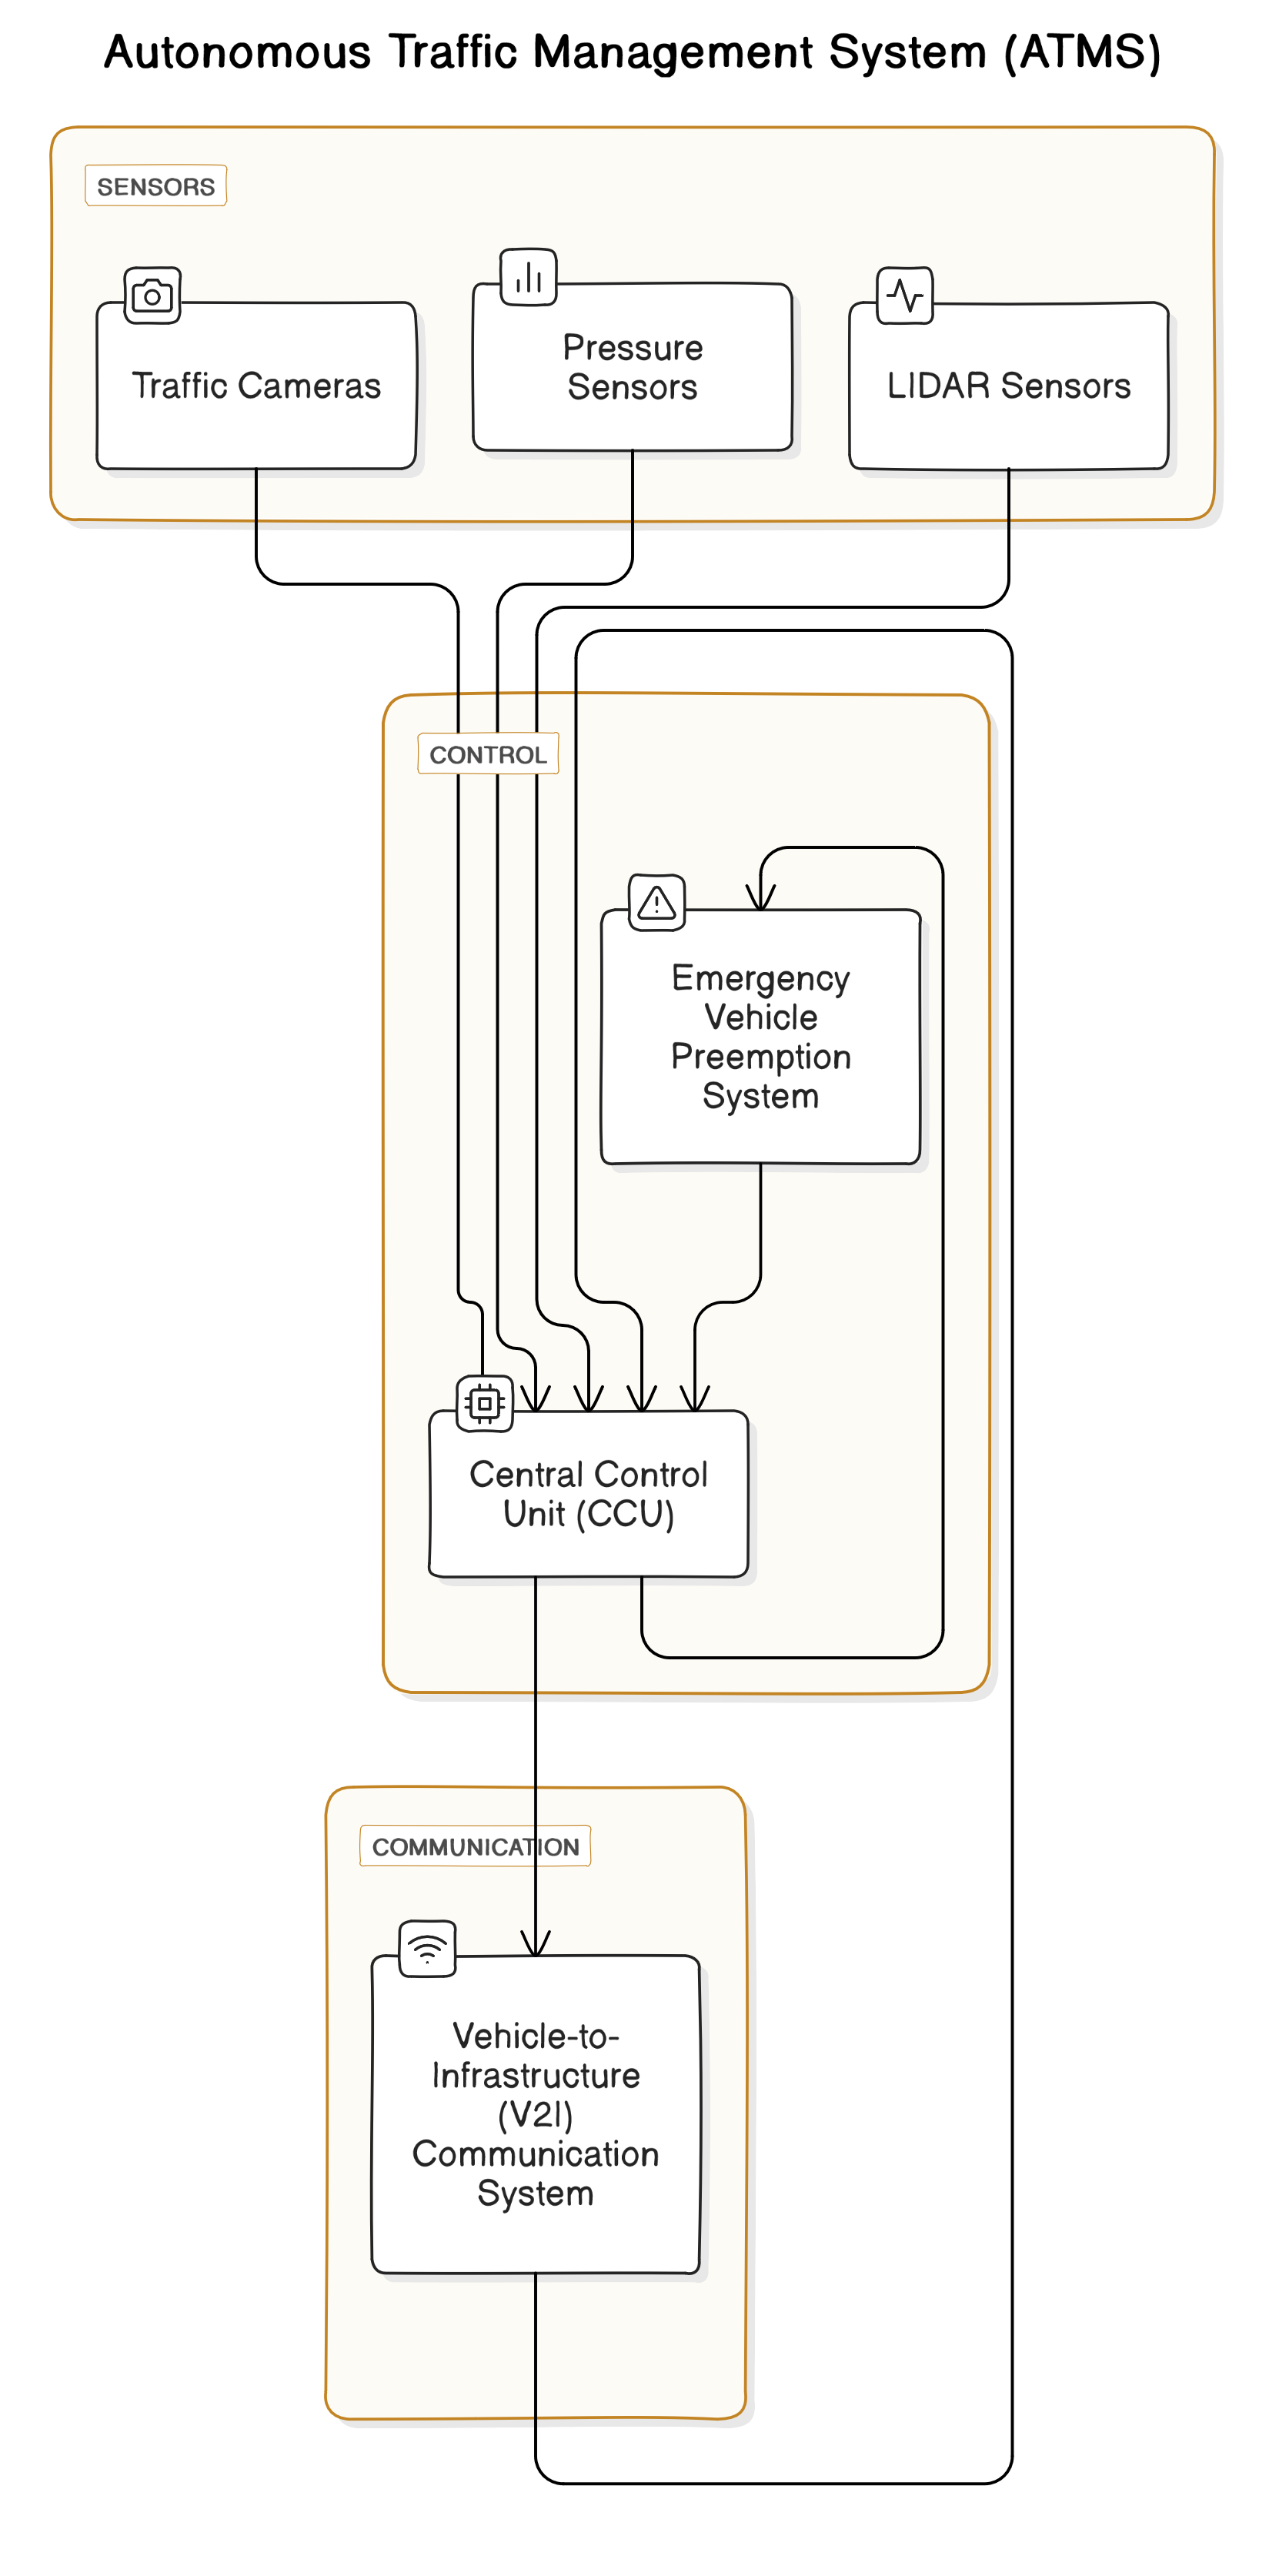
\includegraphics[width=350px, height=550px]{e.png}}
    \parbox{0.8\textwidth}{ 
        \centering
        \textbf{Figure : Autonomus Traffic Management System Design}
    }
\end{center}


\section*{Impact on Real Life}

The implementation of the Autonomous Traffic Management System (ATMS) in urban environments has profound implications for everyday life, particularly in densely populated areas where traffic congestion is a major concern. By utilizing microcontrollers and microprocessors, the system can efficiently manage traffic flow at intersections, significantly reducing the time vehicles spend idling and the overall number of stops. This improvement not only enhances the driving experience by decreasing travel times but also contributes to environmental sustainability by lowering fuel consumption and reducing emissions. Additionally, the system’s ability to prioritize emergency vehicles ensures quicker response times, which can be crucial in saving lives during critical situations. The integration of ATMS with Vehicle-to-Infrastructure (V2I) communication further enhances road safety, particularly as autonomous vehicles become more common, by reducing the likelihood of accidents through coordinated traffic signals. Moreover, the system's adaptability to future technologies and urban expansion means that its benefits will continue to grow, supporting the evolution of smart cities. By optimizing traffic management and improving overall safety and efficiency, the ATMS has the potential to transform urban living, making cities more livable, sustainable, and responsive to the needs of their residents.

\section*{Complex Problem-Solving Questions}

\begin{enumerate}
    \item \textbf{Does problem-solving need in-depth engineering knowledge?} \\
    Yes, designing the Autonomous Traffic Management System (ATMS) requires in-depth knowledge of embedded systems, traffic management algorithms, vehicle communications, and real-time data processing.

    \item \textbf{Does the problem-solving involve wide-ranging or conflicting technical, engineering, and other issues?} \\
    Yes, it involves various challenges, including real-time decision-making, conflicting stakeholder interests (commuters vs. environmental organizations), and integrating both human-driven and autonomous vehicles.

    \item \textbf{Is the solution well-known or require abstract thinking and analysis to formulate?} \\
    The solution involves abstract thinking and cutting-edge technology integration, including autonomous vehicles, real-time data analysis, and eco-friendly optimizations, making it a relatively new and evolving approach.

    \item \textbf{Does the problem-solving involve infrequently encountered issues?} \\
    Yes, issues like coordinating autonomous and human-driven vehicles in real-time and optimizing traffic for diverse conditions and vehicles are not frequently encountered in traditional systems.

    \item \textbf{Does problem-solving need adherence to standards and codes of practice?} \\
    Yes, safety and communication standards (such as V2I communication protocols) must be adhered to for system effectiveness and interoperability.

    \item \textbf{Does the problem-solving involve stakeholders with conflicting technical requirements?} \\
    Yes, balancing the needs of city authorities, transportation agencies, commuters, autonomous vehicle manufacturers, and environmental organizations requires careful consideration and conflict resolution.

    \item \textbf{Does solving involve interdependence between sub-problems or component parts?} \\
    Yes, traffic optimization, emergency preemption, and autonomous vehicle coordination are interdependent, requiring integrated solutions to ensure smooth operations.
\end{enumerate}



\section*{Conclusion}
The Autonomous Traffic Management System (ATMS) offers an intelligent approach to managing traffic at intersections, enhancing overall efficiency while reducing environmental impact. Looking ahead, the system could be expanded to cover additional intersections and integrated with machine learning techniques to further improve traffic prediction and management.

\end{document}
